\documentclass[12pt]{article}
\usepackage[a4paper, total={7in,10in}]{geometry}
\usepackage{polyglossia}
\usepackage{ragged2e}
\usepackage{amsmath}
\usepackage{amssymb}
\usepackage{microtype}
\usepackage{graphicx}
\let\ORIincludegraphics\includegraphics
\renewcommand{\includegraphics}[2][]{\ORIincludegraphics[scale=0.65,#1]{#2}}
\usepackage{changepage}
\usepackage{hyperref}
\usepackage{cancel}
\graphicspath{{./images/}}
\setmainlanguage{russian}
\setotherlanguage{english}
\newfontfamily\russianfont[Script=Cyrillic]{Times New Roman}
\newfontfamily\englishfont{Times New Roman}
\setlength{\parindent}{0em}
\setlength{\parskip}{6pt}

\def\posl#1#2{\{#1_{#2}\}}
\DeclareMathOperator*{\sh-like}{\sinh-like}
\DeclareMathOperator*{\ch-like}{\cosh-like}
\DeclareMathOperator*{\th-like}{\tanh-like}
\DeclareMathOperator*{\cth-like}{\coth-like}
\DeclareMathOperator*{\tg-like}{\tan-like}
\DeclareMathOperator*{\ctg-like}{\cot-like}
\DeclareMathOperator*{\arctg-like}{\arctan-like}
\DeclareMathOperator*{\arcctg-like}{\arctan-like}

\begin{document}
  \tableofcontents
  \pagebreak
  \section{Введение в теорию обыкновенных дифференциальных уравнений(ТОДУ) Лекция №1, дата 24.09.24}
  \subsection{Предмет и задачи курса ДУ}
  \subsection*{Обыкновенные дифференциальные уравнения}
  \begin{enumerate}
    \item Классификация и методы получение аналитических решений ОДУ, в том числе и в CAE системах(Mapple,MatLab)
    \item Элементы качественного анализа
    \item Основные численные методы
  \end{enumerate}
  ТОДУ позволяет изучать всевозможные эволюционные процессы: обладающие свойствами:
  \begin{enumerate}
    \item Детерминированности (состояние в прошлом и будущий ход событий однозначно определяются
    состоянием системы в настоящем)
    \item Конечномерности(число параметров необходимых для описания поведения системы конечно)
    \item Дифференцируемости(фазовое пространстро имеет структуру дифференцируемого многообразия,
    а его изменение описывается дифференцируемыми функциями)
  \end{enumerate}
  \subsection{Объект изучения - обыкновенные дифференциальные уравнения n-порядка}
  $F(x,y,y',\dots,y^{(n)})=0$\\
  $x \in I \sqsubset R,y(x)$ - подлежит определению, n-порядок ДУ\\
  \[y^{(n)}=f(x,y,y',\dots,y^{(n-1)})\] \\
  ОДУ n-порядка разрешенно относительно производной (n)-го порядка
  \subsection*{ОДУ первого порядка выраженное относительно производной}
  \[y'=f(x,y),D,y(x),I\]\\
  D-область определения f(x,y)($D \sqsubseteq R^2),x \in I, I \sqsubseteq R$\\
  Замечание(часто в ТОДУ)$\overset{.}{x}=\varphi(t,x),D,x(t),I$\\
  \underline{Определение: } Пусть f(x,y) действительнозначная функция действительных переменных x и y
  c областью определения $D \sqsubseteq R^2$. функция y(x)($x \in I, I\sqsubseteq R$)
  для которой всюду на I выполняется равенство y'=f(x,y) называется решением дифференциального уравнения
  (1). График решения называется интегральной кривой.\\
  Пример 1: y'=y-x,$R^2,1+x+C \; e^x,R$\\
  \begin{gather*}
    y'=y-x,y(x)-? \; x-\text{парм.}\\
    \text{Ввд } z(x)=y(x)-x\\
    y'=\frac{dy}{dx}\\
    x'=y'-1\\
    z'+1=z\\
    z'=z-1\\
    \frac{dz}{dx}=(z-1)\\
    \int \frac{dz}{z-1}=\int dx => C+ln(z-1)=x+C\\
    ln|z-1|=x+c\\
    |z-1|=e^{x+C}\\
    z-1=e^x\\
    z=Ce^x+1\\
    y(x)-x=Ce^x+1\\
    y(x)=x+1+Ce^x
  \end{gather*}
  \subsection{Элементы качественного анализа ОДУ, лекция №2, дата 01.10.24}
  Исследование однопараметрической группы $g^tx$ диффеоморфизмов, многообразия пространст M, векторных полей на M и связей между ними. \par\noindent
  \begin{center}
    \includegraphics[scale=0.5]{"1.3.1.png"}
  \end{center}
  \begin{center}
    \includegraphics[scale=1]{"1.3.2.png"}
  \end{center}
  \subsubsection*{Теорема Существования}\label{th:1.3.1}
  Если f(x,y) непрерывна в D, то для всякой точки ($x_0,y_0)\in D$ существует
  решение y(x),$(x \in I)$, уравнения y'=f(x,y) такое, что $x_0 \in I \text{ и } y(x_0)=y_0$ \par\noindent
  \underline{Пример 2:}\\
  y'=$2|y|^\frac{1}{2},\mathcal{R}^2,(x-c)^2,0,\mathcal{R}$\\
  y($x_0)=y_0,C=x_0-\sqrt{|y_0|},y_0>0(y_0<0)$
  \subsubsection*{Теорема единственности}\label{th:1.3.2}
  Если f(x,y) и $\frac{df}{dy}$ непрерывна в некоторой D, то для вской точки ($x_0,y_0) \in D$
  ,существует единственное решение y(x) уравнения y'=f(x,y)$\in D,$существует единственное решение
  y(x) уравнения y'=f(x,y) такое, что $y(x_0)=y_0$\par\noindent
  \underline{Замечание:}(к Примеру 2)\\
  $f(x,y)=2|y|^\frac{1}{2},\frac{df}{dy}=\frac{\varsigma(y)}{\sqrt{|y|}}$, неопределима в точку y=0
  \underline{Замечание:}(к Примеру 1)\\
  $f(x,y)=y-x$, непрерывна и $\frac{df}{dy}=1$-непрерывна на D.\\
  Всякая точка ($x_0,y_0$)принадлежит только одному решению\\
  $x(t)=1+t+Ce^t, \; C=(x_0-t_0-1)e^{-t_0}$
  \subsection{Оду первого порядка выраженное относительно производной. Задача Коши}
  $\Bigg\{\begin{aligned}
    \overset{.}{x}=\varphi(x,t)\\
    x(t_0)=x_0, t \in \mathcal{R}
  \end{aligned}$\\
  $\Bigg\{\begin{aligned}
    y'=f(y,x)\\
    y(x_0)=y_0,x \in I \sqsubset \mathcal{R}
  \end{aligned} \; I:(a,b),[a,b),\dots \; -\infty \leq a < b \leq +\infty$\\
  \underline{Пример: Задача Коши}\\
  $\Bigg\{\begin{aligned}
    y'=y-x\\
    y(0)=1
  \end{aligned}$
  \subsection*{Простейшие уравнения и примеры}
  \underline{Пример 1:}Радиоактивного распада (Pp)(размножение бактерий - Рб)\\
  $M=\{x:x>0\}$,x- количества вещества, k>0\\
  M-фазовое пространство(полупрямая)\\
  $\overset{-}{v}=-kx$ или $\overset{.}{x}=-kx \; (Pp)$\\
  $\overset{.}{x}=kx \;$(Рб)
  \subsection*{Рост популяции некоторого изолированного вида}
  \begin{center}
    $y'=ky, \; y,k>0$\\
    Фазовый портрет\\
    \includegraphics[scale=0.7]{"1.4.1.png"}\\
    Анализируя фазовый портрет видим, что в этой модели популяция растет неограниченно.\\  
  \end{center}
  %тут пик должен быть%
  \underline{Замечание:} Закон Ньютона. $T'=-k(T-T_0),k>0$
  \subsection*{Фазовый портерт}
  Фазовый портерт фиксирует лишь качественно поведение системы. \\
  Как изменить дифференциальное уравнение анализируя фазовый портрет? \\
  Предположим, что окрестность может обеспечить существование не более
  $y_e$ особей популяции.\\
  Очевиден неограниченный рост популяции должен быть чем то остановлен, одна
  из возможностей ввести аттрактор.
  \begin{center}
    \includegraphics[scale=0.7]{"1.4.2.png"}\\
    \includegraphics[scale=0.7]{"1.4.3.png"}
  \end{center}
  \subsection*{Автономные уравнения}
  \underline{Определение: } Уравнение y'=f(y),$y \in S \sqsubseteq \mathcal{R},D=\mathcal{R}xS$
  называется автономным\\
  Основное свойство: Если y(x) - решение автономного уравнения y'=f(y), где x $\in I,y \in S$,
  то $\varphi(x)=y(x+c)$ для всякой C $\in R$, является решением $\varphi'=f(\varphi)$,
  где x$\in I,\varphi \in S$\\
  \begin{center}
    Семейства интегральных кривых, получается сдвигами
  \end{center}
  \underline{Замечание:} Уравнение y'=f(y,x) может быть сведено к исскуственной автономной системе
  заменой x'=1(точки равновесия отсутствуют)\\
  \underline{Замечание:} качественное поведение определяется качественным поведением
  каждого индивидуального решения, а оно определяется f(y).\\
  Если f(y)$\not =$ 0, то решение y(x) возрастает или убывает.\\
  Если f(y)=0, то решение y(x)$\equiv $const.\\
  Эти свойства удобно изображать на фазовой прямой y.\\
  \underline{Определение: } Если f(x)=0, то y=c - неподвижная точка(стационарная, точка равновесия).
  \begin{center}
    \includegraphics{"1.4.4.png"}
  \end{center}
  Если число неподвижных точек конечно, существует только конечное число "различных"
  фазовых портертов.
  \begin{center}
    Если y(x)$\not =$C, то y(x) возрастает или убывает.\\
    \includegraphics[scale=0.7]{"1.4.5.png"}

  \end{center}
  \subsection{Классификация неподвижных точек. Лекция №3, дата 08.10}
  \begin{center}
    \includegraphics{"1.5.1.png"}
  \end{center}
  \underline{Определение: } Дифференциальные уравнения имеющие один и тот же фазовый портрет
  считаются качественно эквивалентными, если они имеют одинаковое количество неподвижных точек
  ,одинакового характера и последовательности.
  \subsection{Интегральные кривые. Поле направлений}
  \underline{Определение: }График решения y=y(x) дифференциального уравнения y'=f(x,y)
  ($x \in I, I \sqsubseteq \mathcal{R}$) называется интегральной кривой.\\
  \underline{Определение: } Множество всех отрезков в любых точках в расширенной фазовой плоскости
  называют полем направлений.
  \begin{center}
    \includegraphics{"1.6.1.png"}
  \end{center}
  \underline{Пример:}
  \begin{center}
    \includegraphics[scale=0.7]{"1.6.2.png"}
  \end{center}
  \section{Обыкновенные дифференциальные уравнения первого порядка.Разрешенные относительно производной}
  \begin{center}
    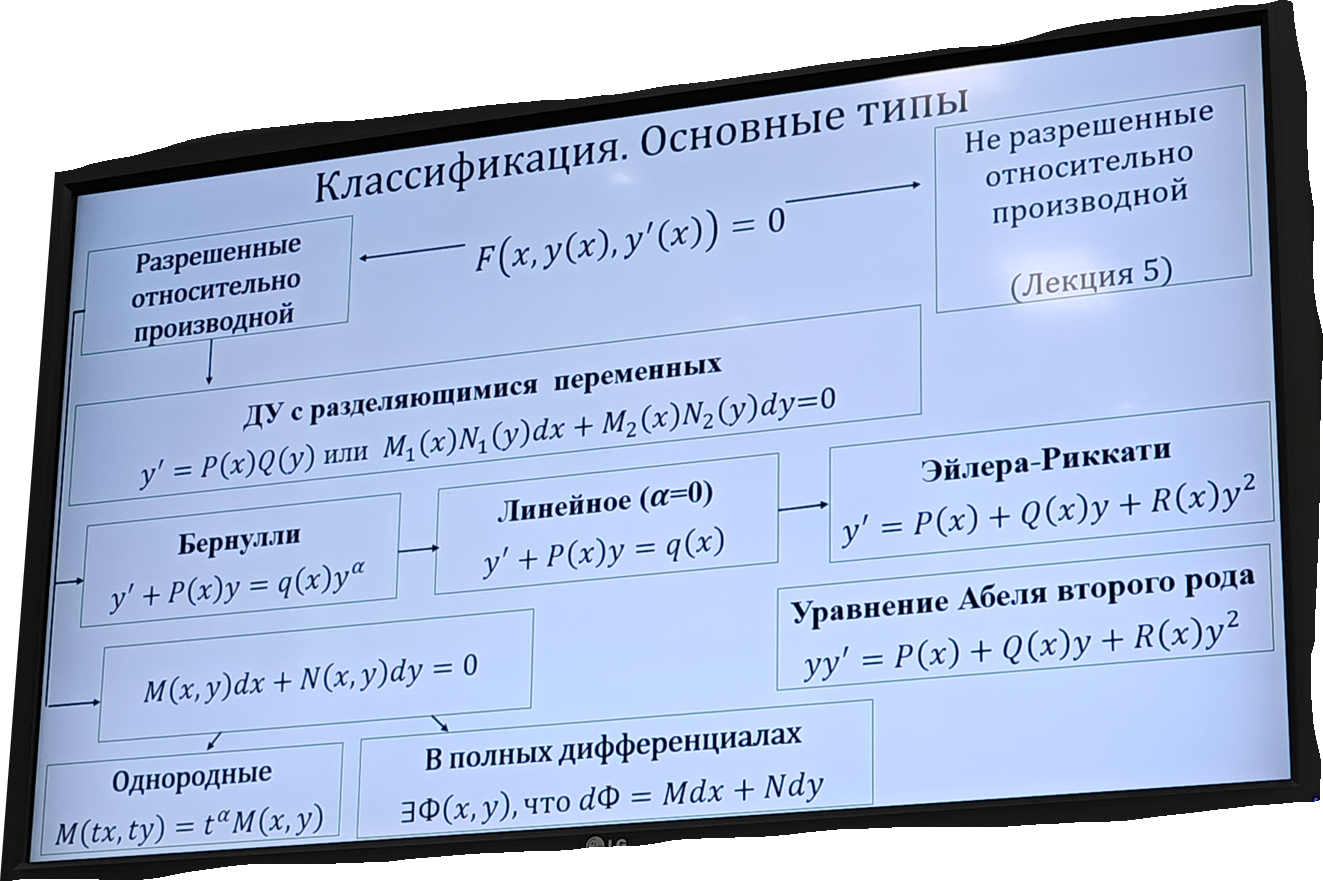
\includegraphics[scale=0.5]{2.1.1.png}
  \end{center}
  \subsection{Линейные ДУ I порядка(уравнение Бернулли)}
  \begin{center}
    $y'+p(x)y=q(x)(y'+p(x)y=q(x)y^2)$
  \end{center}

  \begin{minipage}{0.48\textwidth}
    Метод вариаций постоянной\\
    \begin{enumerate}
      \item $\frac{dy}{y}=-p(x)y$
      \item C(x)-?\\
      y=$C(x)e^{-\int p(x)dx}$
      \item C(x)=$\int q(x)e^{\int p(x)dx}dx$\\
      y(x)=$(\int q(x)e^{\int p(x)dx}+C)e^{-\int p(x)dx}$
    \end{enumerate}
    \underline{Пример 2:} $(2x+1)y'=(4x+2y)$
  \end{minipage}
    \hfill
  \begin{minipage}{0.48\textwidth}
    Метод замены\\
    y(x)=u(x)v(x)\\ 
    где v(x) - решение однородного линейного ДУ\\
    \\
    v'(x)+p(x)v(x)=0\\
    u'(x)v(x)=q(x)\\
    \underline{Пример 3:} $(2e^y-x)y'=1$
  \end{minipage}
\end{document}